\documentclass[12pt,a4paper]{article} % albo book
\usepackage{polski}
\usepackage{fontspec}
\usepackage{graphicx}
\usepackage[center]{caption}
\usepackage{pdfpages}
\setmainfont{Times New Roman}


\linespread{1.5}

\renewcommand{\figurename}{Rys.}


\usepackage{geometry}
\newgeometry{tmargin=2cm, bmargin=2cm, lmargin=2cm, rmargin=2cm}
\newcommand{\noaka}{\hspace{-6mm}}
\newcommand{\aka}{\hspace{1cm}}
\newcommand{\citate}[1]{$^{[\ref{#1}]}$}

\newcounter{questionsCount}
\setcounter{questionsCount}{1}
\newcommand{\question}[1]{\textcolor{red}{\mbox{Pytanie}~\arabic{questionsCount}:~#1 \addtocounter{questionsCount}{1}}}

\pagenumbering{gobble}
\usepackage{xcolor}
\usepackage{listings}

\renewcommand{\lstlistingname}{Fragment kodu}

%New colors defined below
\definecolor{codegreen}{rgb}{0,0.6,0}
\definecolor{codegray}{rgb}{0.5,0.5,0.5}
\definecolor{codepurple}{rgb}{0.58,0,0.82}
\definecolor{backcolour}{rgb}{0.95,0.95,0.92}

%Code listing style named "mystyle"
\lstdefinestyle{mystyle}{
  backgroundcolor=\color{backcolour}, commentstyle=\color{codegreen},
  keywordstyle=\color{magenta},
  numberstyle=\tiny\color{codegray},
  stringstyle=\color{codepurple},
  basicstyle=\ttfamily\footnotesize,
  breakatwhitespace=false,         
  breaklines=true,                 
  captionpos=b,                    
  keepspaces=true,                 
  numbers=left,                    
  numbersep=5pt,                  
  showspaces=false,                
  showstringspaces=false,
  showtabs=false,                  
  tabsize=2
}
\lstset{style=mystyle}


\pagenumbering{arabic}
\begin{document}

\includepdf[pages=-]{images/strona_tytułowa.pdf}

%%%%%%%%%%%%%%%%%%%%%%%%%%%%%%%%%%%%%%%%%%%%%%%%%%%%%
%%%%%%%%%%%%%%% IDEA PROJEKTU / WSTĘP %%%%%%%%%%%%%%%
%%%%%%%%%%%%%%%%%%%%%%%%%%%%%%%%%%%%%%%%%%%%%%%%%%%%%
\section{Idea projektu/Wstęp}


%%%%%%%%%%%%%%%%%%%%%%%%%%%%%%%%%%%%%%%%%%%%%%%%%%%%%
%%%%%%%%%%%%% IDEA DZIAŁANIA APLIKACJI %%%%%%%%%%%%%%
%%%%%%%%%%%%%%%%%%%%%%%%%%%%%%%%%%%%%%%%%%%%%%%%%%%%%
\section{Idea działania aplikacji}

\aka Działanie aplikacji polega na realizowaniu kolejnych poziomów. Każdy poziom zawiera opis działania układu oraz opis połączenia  komponentów elektronicznych. Użytkownik ma możliwość zarejestrowania oraz zalogowania się do aplikacji w~celu zapisania postępu  w~"chmurze".
Na rys. \ref{rys:diagram-przypadków-użycia}  przedstawiony został diagram przypadków użycia, który pokazuje funkcjonalne aspekty aplikacji.  

\begin{figure}[h]
	\centering
	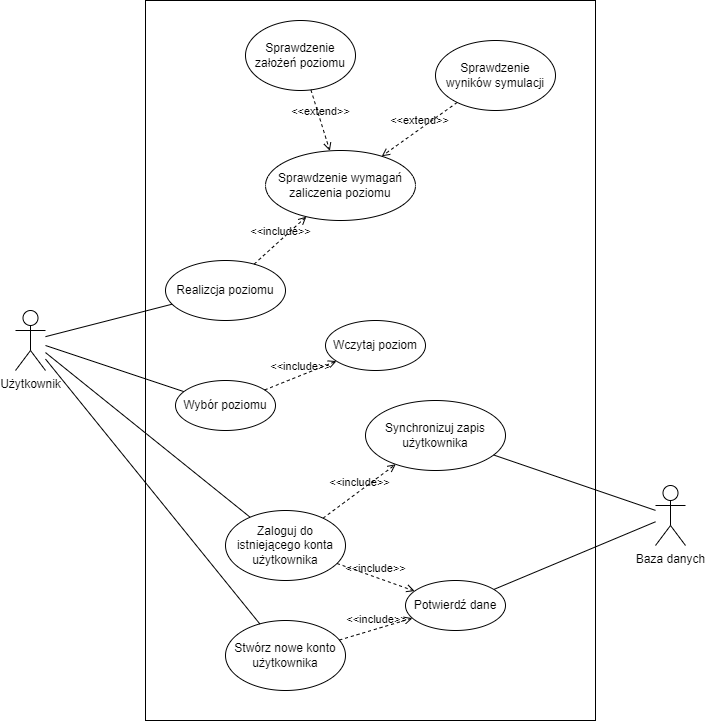
\includegraphics[width=10cm]{images/use_case_diagram.png}
	\caption{Diagram przypadków użycia \\ Źródło: opracowanie własne}
	\label{rys:diagram-przypadków-użycia} %odwołanie do rysunku: \ref{rys:diagram-przypadków-użycia}
\end{figure}
  
\question{moze dodać opis każdego use casa?}

%%%%%%%%%%%%%%%%%%%%%%%%%%%%%%%%%%%%%%%%%%%%%%%%%%%%%
%%%%%%%%%%%%%%%%% PROJEKT APLIKACJI %%%%%%%%%%%%%%%%%
%%%%%%%%%%%%%%%%%%%%%%%%%%%%%%%%%%%%%%%%%%%%%%%%%%%%%
\clearpage
\section{Projekt aplikacji}
\aka Procesor wykonuje instrukcje w~sposób sekwencyjny, więc do zachowania ciągłości renderowania obrazu wymagane jest, by aplikacja zawierała nieskończoną pętlę, w~której jest zawarte sprawdzanie zdarzeń, aktualizowanie aplikacji oraz rysowanie okna \cite{gameprogrammingpatterns}. Schemat blokowy głównej pętli został przedstawiony na rys. \ref{rys:main_loop}. Dodany warunek sprawdzania fokusu okna pozwala na nie wykorzystywanie zasobów sprzętowych, w przypadku gdy okno jest nie aktywne, bądź jest zminimalizowane.

\begin{figure}[h]
	\centering
	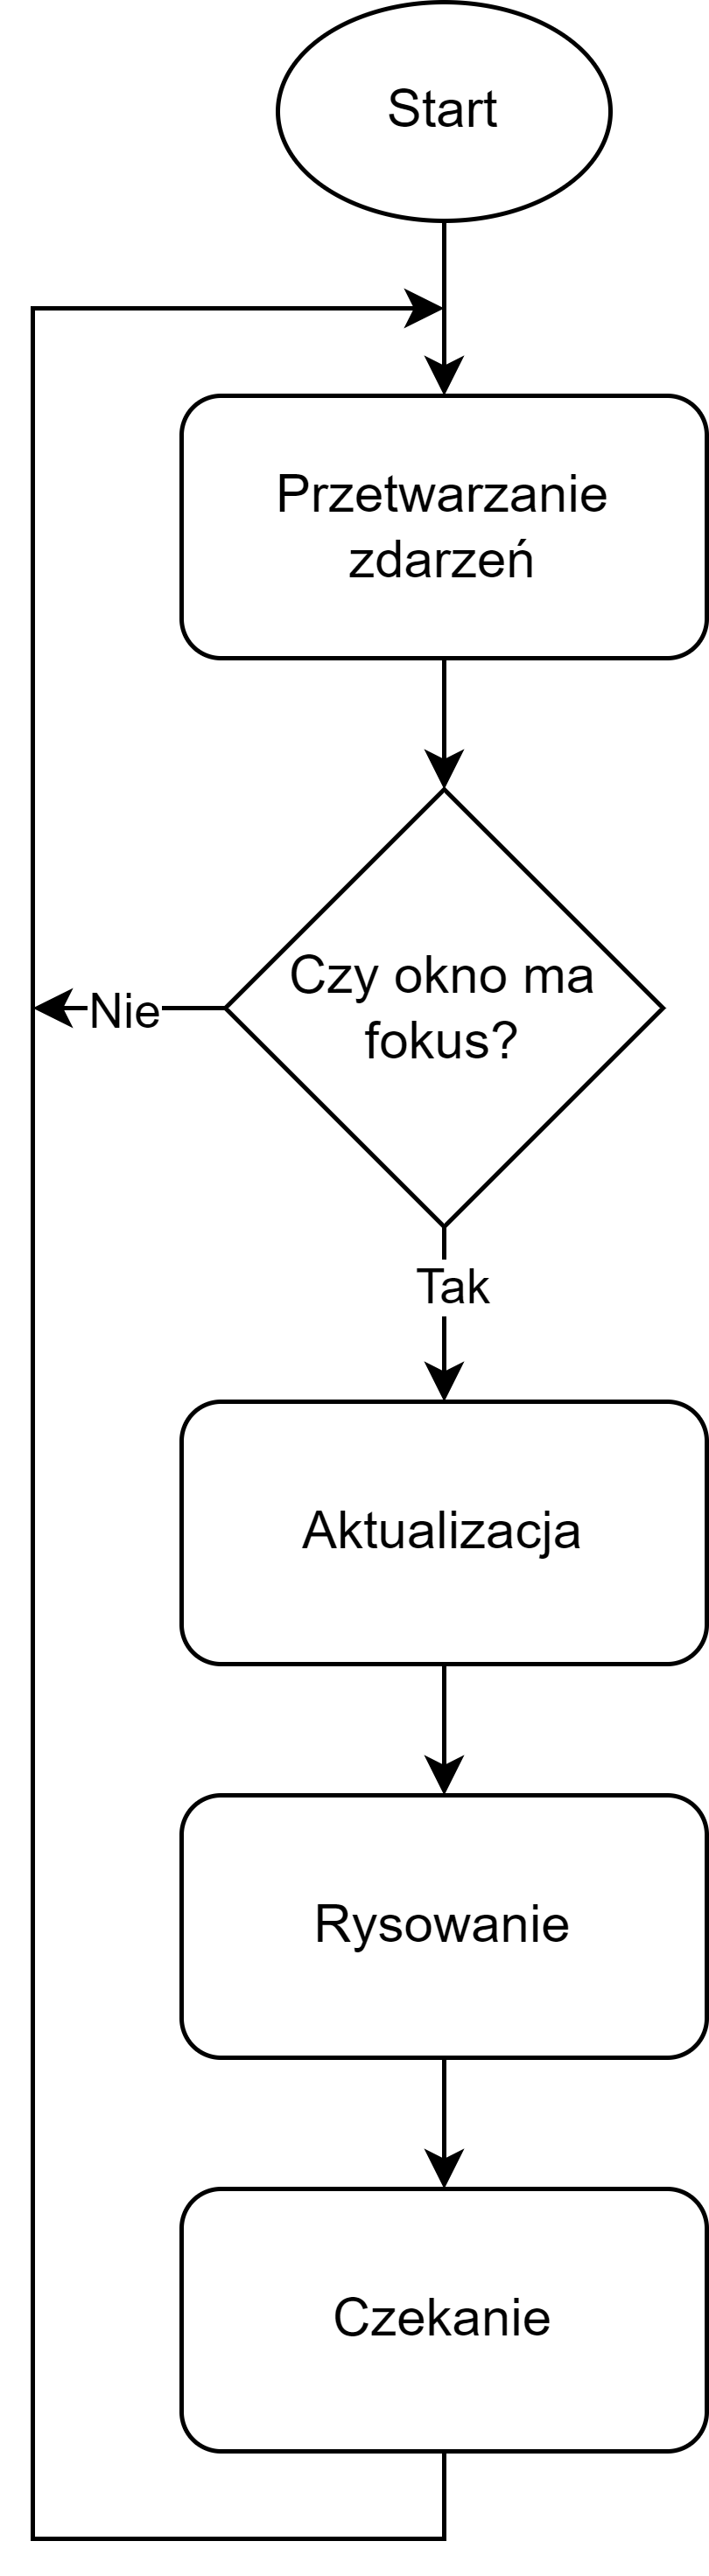
\includegraphics[height=10cm]{images/main_loop.png}
	\caption{Schemat blokowy pętli głównej \\ Źródło: opracowanie własne na podstawie \cite{gameprogrammingpatterns}}
	\label{rys:main_loop}
\end{figure}


\aka Przechodzenie pomiędzy widokami aplikacji zostało zrealizowane w klasie \textit{Game}. Diagram maszyny stanów tej klasy został przedstawiony na rys. \ref{rys:diagram_maszyny_stanów}.
\question{w jaki sposób powinienem odwoływać się do nazw klas/obiektów, kursywą?}


\begin{figure}[h]
	\centering
	\includegraphics[width=15cm]{images/maszyna_stanów_aplikacji.png}
	\caption{Diagram maszyny stanów obiektu klasy \textit{Game} \\ Źródło: opracowanie własne}
	\label{rys:diagram_maszyny_stanów}
\end{figure}



\begin{figure}[h]
	\centering
	\includegraphics[width=15cm]{images/diagram_klas_stanów.png}
	\caption{Uproszczony diagram klas pokazujący dziedziczenie klas dla maszyny stanów obiektu klasy \textit{Game} \\ Źródło: opracowanie własne}
	\label{rys:diagram_klas_stanów}
\end{figure}


\aka Gdy użytkownik ułoży komponenty na planszy, a~następnie wciśnie przycisk sprawdzający zadanie, to aplikacja utworzy plik z~schematem. Następnie aplikacja wykona symulację wykorzystując zewnętrzny, darmowy program \textbf{LTspice} oraz wygenerowany plik.
Rys. \ref{rys:diagrma_sekwencji_symulacji} przedstawia diagram sekwencji zawierający interakcję między obiektami, gdy aplikacja będzie sprawdzała poziom.

\begin{figure}[h]
	\centering
	
\includegraphics[width=15cm]{images/no_image.png}
	\caption{Diagram sekwencji, pokazujący interakcję podczas symulacji \\ Źródło: opracowanie własne}
	\label{rys:diagrma_sekwencji_symulacji}
\end{figure} 

%%%%%%%%%%%%%%%%%%%%%%%%%%%%%%%%%%%%%%%%%%%%%%%%%%%%%
%%%%%%%%%%%%%% IMPLEMENTACJA APLIKACJI %%%%%%%%%%%%%%
%%%%%%%%%%%%%%%%%%%%%%%%%%%%%%%%%%%%%%%%%%%%%%%%%%%%%
\clearpage
\section{Implementacja aplikacji}

\subsection{Wprowadzenie} %???
\aka Główna część aplikacja została zaimplementowana w języku C++, wykorzystując standard ISO C++ 14. 
%Powodem ?
% Aplikacja do poprawnego działania, w celu wykonania symulacji, wykorzystuje zewnętrzny program LTspice. Wykorzystanie zewnętrznego 
Do komunikacji z~zewnętrznym programem wykorzystany został język Python w~wersji 3.12 osadzony w~głównej części aplikacji. Takie rozwiązanie pozwala na bezpośredni dostęp do zasobów wykonywanego kodu w~języku Python przez aplikajcę w~C++. 
Aplikacja została zaimplementowana z~myślą o~systemie operacyjnym Windows, natomiast wykorzystane biblioteki pozwalają na przeniesie na inne systemy operacyjne dystrybucji Linux czy macOS. %?????
\question{not sure}

Wykorzystaną bazą danych jest MySQL.


\subsection{Środowisko oraz narzędzia programistyczne}
\aka Wykorzystanym środowiskiem programistycznym było Visual Studio 2022. Zostały wykorzystane moduły: \textit{Graphics, System, Window} biblioteki SFML \textit{(Simple and Fast Multimedia Library)} opartej o~OpenGL. Wykorzystanie tych modułów pozwala na proste i~wydajne rysowanie okna na ekranie oraz przekazywanie własnych parametrów do strumienia przetwarzania potoku grafiki. Zastosowana została również standardowa biblioteka STL. 

\aka Aplikacja w~celu przekazania i~odebrania danych z~symulacji wykorzystuje bibliotekę Python. Natomiast w~zagnieżdżonej części Python wykorzystuje moduł PyLTSpice do realizacji symulacji oraz moduł ltspice do odczytania obliczonych wartości symylacji.

\aka Do wykonywania zapytań z~bazą danych wykorzystana została biblioteka mysqlx. Baza danych była uruchamiana w środowisku kontenerowym Docker, do inicjalizacji tabel oraz relacji wykorzystany został język SQL. 

ciekawsze mi się wydaje:
- pakowanie/rozpakowywanie danych z db
- coś z poziomem
- fragmenty z symulacji
- jak wygląda płytka
- dodawanie ścieżki
- przykładowy poziom

\begin{lstlisting}[language=C++, caption={awawd \\ Źródło: opracowanie własne}]
  class PopupBox : public sf::Drawable
{
public:
	PopupBox()
	{

	}

private:
	virtual void draw(sf::RenderTarget& target, sf::RenderStates states) const
	{
		target.draw(text, states);
	}

	sf::Font* font;
	sf::Text text;
};
\end{lstlisting}

%%%%%%%%%%%%%%%%%%%%%%%%%%%%%%%%%%%%%%%%%%%%%%%%%%%%
%%%%%%%%%%%%% URUCHOMIENIE APLIKACJI %%%%%%%%%%%%%%%
%%%%%%%%%%%%%%%%%%%%%%%%%%%%%%%%%%%%%%%%%%%%%%%%%%%%
\section{Uruchomienie aplikacji}

%%%%%%%%%%%%%%%%%%%%%%%%%%%%%%%%%%%%%%%%%%%%%%%%%%%%
%%%%%%%%%%%%%%% TESTOWANIE APLIKACJI %%%%%%%%%%%%%%%
%%%%%%%%%%%%%%%%%%%%%%%%%%%%%%%%%%%%%%%%%%%%%%%%%%%%
\section{Testowanie aplikacji}


%%%%%%%%%%%%%%%%%%%%%%%%%%%%%%%%%%%%%%%%%%%%%%%%%%%%
%%%%%%%%%%%%%%%%%%% LITERATURA %%%%%%%%%%%%%%%%%%%%%
%%%%%%%%%%%%%%%%%%%%%%%%%%%%%%%%%%%%%%%%%%%%%%%%%%%%
% literatura
% Odwołanie: \cite{texbook}
\begin{thebibliography}{9}
% dodanie do listy literatury
% \bibitem{texbook}
% Donald E. Knuth (1986) \emph{The \TeX{} Book}, Addison-Wesley Professional.
% dodanie do listy literatury
% \bibitem{lamport94}
% Leslie Lamport (1994) \emph{\LaTeX: a document preparation system}, Addison
% Wesley, Massachusetts, 2nd ed.
\bibitem{gameprogrammingpatterns}
Game Programming Patterns, Robert Nystrom, https://gameprogrammingpatterns.com/game-loop.html
\end{thebibliography}

\end{document}